%
% File naaclhlt2010.tex
%
% Contact: nasmith@cs.cmu.edu

\documentclass[11pt,letterpaper]{article}
\usepackage{naaclhlt2010}
\usepackage{times}
\usepackage{latexsym}
\usepackage{graphicx}
\setlength\titlebox{6.5cm}    % Expanding the titlebox

\title{Optimization of Nearest Neighbors: Run Time and Accuracy}

\author{Kyle Wong \\
  3400 N. Charles St. \\
  Baltimore, MD 21218 \\
  {\tt kwong23@jhu.edu}
  \And
  Tifany Yung \\
  3400 N. Charles St. \\
  Baltimore, MD 21218 \\
  {\tt tyung1@jhu.edu}}

\date{May 12, 2014}

\begin{document}
\maketitle
\begin{abstract}
Ligands can react with a particular receptor in one of three ways: bind and activate the receptor, bind and inhibit the receptor, and not bind at all. Whether a ligand is likely to bind to a receptor can be determined by considering the features such as ligand and receptor shapes, charges, and molecular forces. All of the factors can be accounted via FRED (Fast Rigid Exhaustive Docking) which calculates the Chemgauss4 (cg4) scoring function.

Since the relative positions of both the ligand and receptor affect the likelihood of binding, the FRED scores for 500 receptor frames crossed with each of 710 ligands were taken to create a system for predicting whether a particular ligand will bind with the receptor. These 500 frames were used as the features for feature vectors with the ligands as an instances.

The labeled ligand instances and their 500-FRED-score-long feature vectors were used to train a basic $\epsilon$-sphere, nearest neighbors algorithm with low precision and recall results. The algorithm was then improved by selecting features with information gain and testing with different $\epsilon$ values.  However, the original dataset proved to be too small and limited to get conclusive results.  Synthetic data was then generated for testing and improving the nearest neighbors algorithm.  Then, the nearest neighbors algorithm was improved using a K Means EM (Expectation Maximization) algorithm to cluster the data points with highly positive results.  
\end{abstract}

\section{Introduction}
\subsection{Nearest Neighbor Algorithm}

The $\epsilon$-sphere nearest neighbors algorithm is a close relative of the K-nearest neighbors algorithm; both are clustering algorithms designed with the purpose of categorizing data into a certain number of categories, or labels. As an example, for the ligand-receptor data used, the ligands would be labeled with whether or not they bind with the given receptor.

Clustering algorithms work by using nearby points to determine which cluster or label a given point should be placed in based on the labels of the points around it. The only difference between the above-mentioned $\epsilon$-sphere and K nearest neighbors is how to choose the points around the test point to help determine the test point's label. In the K nearest neighbors algorithm, the number K of points closest to the test point are taken, and the test point is assigned the majority label amongst those points; in the $\epsilon$-sphere algorithm, all points that are within a Euclidean distance of $\epsilon$ or less from the test point are used and the majority label is used as the prediction.

The general structure of the $\epsilon$-sphere clustering algorithm is the same as any machine learning algorithm: teaching the algorithm using a training dataset, and testing the accuracy of the algorithm with a development dataset. During training of $\epsilon$-sphere clustering, the training data points are simply read in and stored. 

During testing, data points are input individually, and the algorithm attempts to predict their label. It does so by taking all data points within Euclidean distance $\epsilon$ of the test point and calculating the majority label amongst those points. The test point is then assigned to that majority label.

There has been some previous research into speeding up K nearest neighbors by using $\epsilon$-sphere. Indyk and Rajeev (1998) first implemented and tested a kd-tree for the $\epsilon$-sphere algorithm and recommended it only for low-dimensional data. More recently, Muja and Lowe attempted to find fast approximates for the nearest neighbors algorithm.

\subsection{Virtual Screening}
For receptor ligand docking, much of the work is done manually by hand where researchers do virtual screening for a given receptor by hand-picking ligands that they believe will likely bind to the receptor.  This process is known to be very slow and labor-intensive.  As such, automated virtual screening is of utmost importance.  However, simply screening a receptor model with a ligand in a docking program such as FRED often results in incorrect estimates of binding affinity.  The assumption is that ligands that bind to a receptor will fit nicely with the receptor and will thus be detected by having a more negative binding score when screened with docking.  However, oftentimes, ligands that do not bind to a receptor sometimes give a more negative binding score for a given receptor pose. Thus, using multiple receptor poses may improve docking calculations (Totrov et. al. 2008).

However, receptor model poses are frequently incomplete as the conformational space of protein shape and flexibility is so large.  This leads to a wide fluctuation in binding affinity score predictions.  One approach for addressing this issue is identifying the relevant receptor modes to identify the correct ensemble of receptor conformations in order to do more accurate virtual screening (Cavasotto 2005).  This leads to the idea of applying the concept of measuring Information Gain on the receptor frame (pose) features in order to select the frames which are truly relevant.

\section{Data}
The data used for this project includes Ligand/receptor binding data obtained from the Data Management Systems lab. The data consists of 710 labeled ligands that were screened with FRED across 500 frames of a receptor to get Chemgauss4 (cg4) scores. Each receptor frame represents the pose of a receptor at a different time.  10 of the ligands were known to actively bind with the receptor while the other 700 ligands were known to not have binding activity with the receptor.

\section{Methods}
\subsection{Algorithm Selection}
For this project, we assumed that the different frames of the receptor would capture different characteristics of ligands required for the ligand to bind to the receptor.  Therefore, since we had 500 frame data points for each ligand, we chose to do the $\epsilon$-sphere nearest neighbors algorithm under the idea that if two ligands had similar binding scores for the same frames, they would be functionally similar.  Thus, they would have a low Euclidean distance in terms of the frame FRED cg4 scores.

There are a variety of characteristics that can help a ligand to bind to a receptor including: electrostatics forces, solvation and desolvation effects, hydrophobic interactions, bond stretching, dihedral energy terms, hydrogen bonds, and many other factors.  Therefore, our idea was that ligands that bound to the receptor would score similarly to other binding ligands.  And in the same way, non-binding ligands would score similarly to non-binding ligands.  So using the $\epsilon$-sphere nearest neighbors algorithm would help us to identify regions in the frame-ligand score space that corresponded to binding ligands.

\subsection{Algorithm Optimization}
Since some of the receptor frames (the features) may not provide useful and accurate information about ligand binding potential, we decided to try to use a measure of Information Gain to select the best frames for distinguishing whether a ligand would bind or not.  Since we had many frames, there was thus a high dimensionality, so reducing the number of features using Information Gain would also help overcome the "Curse of Dimensionality."  

Since the nearest neighbor algorithm requires iterating over all the training points for every single prediction, we considered creating a KD-Tree data structure to more quickly identify the nearest points.  However, upon further research we realized that KD-trees are not helpful in high-dimensional spaces.  For example, one general rule is that if the dimensionality is k, the number of points in the data, N, should be N much greater than $2^k$. If this is not the case, then a KD-tree will simply evaluate nearly all the points in the tree, and the efficiency is no better than exhaustive search (Goodman et al. 2004).  And in our case, we have $k=500$ and $N=710$ in which case using a KD-tree might even be slower than just exhaustive search.

Thus, we instead implemented a Lambda-Means approach where we would use EM (Expectation Maximization) to cluster points that were close together in terms of Euclidean distance.  Then, when predicting, we would first compare to the prototype vectors and then would only need to compare to the points within that cluster to find the majority of labels of points within the distance $\epsilon$.  In a sense, this approach would be like sorting the training points into different buckets to speed up prediction time by ignoring points that have an average distance that is further away.  This would give us a way to improve the slow runtime of the nearest neighbor algorithm which normally exhaustively must check against all of the training points while not sacrificing accuracy.

\section{Problems Encountered - Data}
\subsection{Ligand Data Problems}
One major setback was the loss of data from the Data Management Systems lab (DAMSL) due to the crash of two RAID Array Controllers.  Thus, this projected was limited in its data to only 10 positive binding ligand instances and only 690 negative non-binding ligand instances.  This proved difficult for splitting the data into dev and train data.  We decided to do a 80\% train 20\% development data split, but that still only have us 8 positive training ligand examples and only 2 positive development testing ligand examples.  Furthermore, due to the DAMSL data loss, we were unable to get more data for testing.  

As for the data itself, it was difficult to find a good optimization.  This seems to be a result of the FRED cg4 scores themselves as the data is not highly indicative of being able to distinguish between positive binding ligands and negative non-binding ligands.  In particular, when we performed statistics on the data, we found that the average FRED score for positive binding ligands and negative non-binding ligands was about the same at a value of around -6.5 and even their standard deviation was about the same of about 1.35

\subsection{Synthetically Generated Data - Ball}
In order to create a more helpful dataset, we generated a dataset called "ball" under the idea that positive binding ligands would have an average binding score of -8 with standard deviation of 1 and that negative non-binding ligands would have an average binding score of -6 with standard deviation of 1.  This synthetic dataset would thus allow us to test our algorithm knowing that the classification would be possible while still having points that overlapped between these two ball regions.

Further, we created this dataset with 50 positive binding ligand instances and with 650 negative non-binding ligands.  This would help us to have a larger number of positive training and development testing examples for evaluating our $\epsilon$-sphere, nearest neighbors algorithm.  We still opted to do a 80\% train 20\% development data split.

We wrote three python scripts to do this: 

\begin{enumerate} 	
	\item csvgen.py to write a comma separated value set similar to what FRED docking would give: compoundstate-id, result (1 or 0), frame-id, FRED cg4 score
	\item keygen.py to format the csv into the same format as data files from class where each line represents a ligand instance with the frames being the features listed
	\item dev.py to split the data into 80\% train 20\% development data
\end{enumerate}

\section{Results}
The algorithm accuracy, precision, recall, and run time in milliseconds for the K-means algorithm is shown below for when all features are used and when only the fifty with the highest information gain are used.

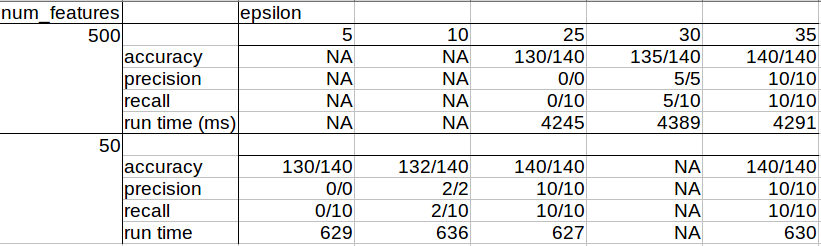
\includegraphics[width=75mm]{formattedData.png}

- what tests did we run

- what do these results mean

\section{Future Work}


\section{Comparison}

The original project proposal suggested three milestones for the optimization of nearest neighbors: minimum, expected, and stretch deliverables. The minimum deliverable was to implement a functional $\epsilon$-sphere nearest neighbor algorithm to predict whether or not a ligand will potentially respond and bind to a given receptor and to implement feature selection via information gain. This implementation was achieved and presented in the class SphereNearestNeighborPredictor.java in the "sphere" package of the "neighbors" project; the results and analysis of the run time and accuracy of this implementation is provided above in the Results section.

The expected deliverable was to implement a faster $\epsilon$-sphere algorithm by using divide-and-conquer in lieu of a linear search for the $epsilon$ closest points to a test point, similar to a kd tree. However, this was not implemented because it was found via additional research (Indyk and Rajeev) that usage of kd trees in higher dimensions are no better than brute-force search since most nodes in the kd tree would need to be evaluated anyways. Therefore, this deliverable was not implemented.

The "Would like to achieve" deliverable was to implement a K-means approach of clustering the training data points by euclidean distance in order to speed-up the time of searching for nearest neighbors.  We finished this deliverable and implemented it in the class KMeansSpherePredictor.java in the "sphere" package of the "neighbors" project. The results and analysis of the runtime improvement and accuracy of this implementation is provided above in the Results section.


\section{Junk}


\begin{thebibliography}{}
\bibitem[\protect\citename{Cavasotto, Claudio N., Julio A. Kovacs, and Ruben A. Abagyan.}2005] {Cavasotto, Claudio N., Julio A. Kovacs, and Ruben A. Abagyan.: 05} Cavasotto, Claudio N., Julio A. Kovacs, and Ruben A. Abagyan.
\newblock Representing receptor flexibility in ligand docking through relevant normal modes.
\newblock {\em Journal of the American Chemical Society}, 127.26 (2005): 9632-9640.

\bibitem[\protect\citename{Cover, Thomas, and Peter Hart.}1967]{Cover, Thomas, and Peter Hart: 67} Cover, Thomas, and Peter Hart.
\newblock 1967.
\newblock Nearest neighbor pattern classification.
\newblock {\em Information Theory, IEEE Transactions}, 13(1):21-27.

\bibitem[\protect\citename{Fukunaga, Keinosuke, and Patrenahalli M. Narendra.}1975] {Fukunaga, Keinosuke, and Patrenahalli M. Narendra: 75} Fukunaga, Keinosuke, and Patrenahalli M. Narendra.
\newblock 1975.
\newblock A branch and bound algorithm for computing k-nearest neighbors.
\newblock {\em Computers, IEEE Transactions}, 100(7): 750-753.

\bibitem[\protect\citename{Goodman, Jacob E., and Joseph O'Rourke.}2004]{Goodman, Jacob E., and Joseph O'Rourke: 04} Goodman, Jacob E., and Joseph O'Rourke.
\newblock 2004.
\newblock Handbook of discrete and computational geometry.
\newblock {\em CRC press}, 2004.

\bibitem[\protect\citename{Indyk, Piotr, and Rajeev Motwani.}1998] {Indyk, Piotr, and Rajeev Motwani: 98} Indyk, Piotr, and Rajeev Motwani.
\newblock 1998.
\newblock Approximate nearest neighbors: towards removing the curse of dimensionality.
\newblock {\em Proceedings of the thirtieth annual ACM symposium on Theory of computing.}

\bibitem[\protect\citename{Muja, Marius, and David G. Lowe.}2009] {Muja, Marius, and David G. Lowe: 09} Muja, Marius, and David G. Lowe.
\newblock Fast Approximate Nearest Neighbors with Automatic Algorithm Configuration.
\newblock {\em VISAPP}, 2009.

\bibitem[\protect\citename{Totrov, Maxim, and Ruben Abagyan.}2008] {Totrov, Maxim, and Ruben Abagyan.: 08} Totrov, Maxim, and Ruben Abagyan.
\newblock Flexible ligand docking to multiple receptor conformations: a practical alternative.
\newblock {\em Current opinion in structural biology}, 18.2 (2008): 178-184.


\end{thebibliography}

\end{document}
